\section{Introduction}

%% Background
Wide-area streaming analytics are becoming pervasive, especially with the
emerging class of Internet of Things (IoT) applications.  Large cities such as
London and Beijing have deployed millions of cameras for surveillance and
traffic control~\cite{skynet, london.surveillance}. Buildings are increasingly
equipped with a wide variety of sensors to improve energy efficiency and
occupant comfort~\cite{krioukov2012building}. Geo-distributed infrastructure,
such as content delivery networks (CDNs), analyzes requests from machine logs
over the globe~\cite{mukerjee2015practical}. These applications need to
transport, distill, and process streams of data across the wide area in real
time.

Although existing stream processing systems, such as
Storm~\cite{toshniwal2014storm}, Spark Streaming~\cite{zaharia2013discretized},
and VideoStorm~\cite{zhang2017live}, can handle large streams of data, they are
designed to work within a single cluster, where the network is not the
bottleneck.  In contrast, the wide area network (WAN) has limited
bandwidth~\cite{hsieh17gaia, vulimiri2015global}. Moreover, WAN bandwidth growth
has been decelerating for many years~\cite{global2016telegeography} while
traffic demands are growing at a staggering rate~\cite{index2013zettabyte}.

Limited WAN bandwidth makes it neither practical nor efficient to back-haul all
data to a central location.  Recent research on WAN-aware systems promotes
pushing computations towards the edge~\cite{rabkin2014aggregation,
  satyanarayanan2009case}. However, communication is not entirely avoidable:
$(i)$ some analytical jobs require joining or aggregating data from multiple
geo-distributed sites~\cite{pu2015low, viswanathan2016clarinet}; $(ii)$ the edge
can benefit substantially from central computing resources such as GPUs and
TPUs~\cite{abadi2016tensorflow} in the cloud; and $(iii)$ end devices, such as
cameras and mobile phones, still suffer from limited bandwidth in last-hop
wireless links when running processing on nearby edge
infrastructure~\cite{abari2017enabling, zhang2015design}.

When facing insufficient bandwidth, application developers need to make a
decision within the design space of data fidelity versus freshness, as
illustrated in \autoref{fig:intro}.

\begin{figure}
  \centering
  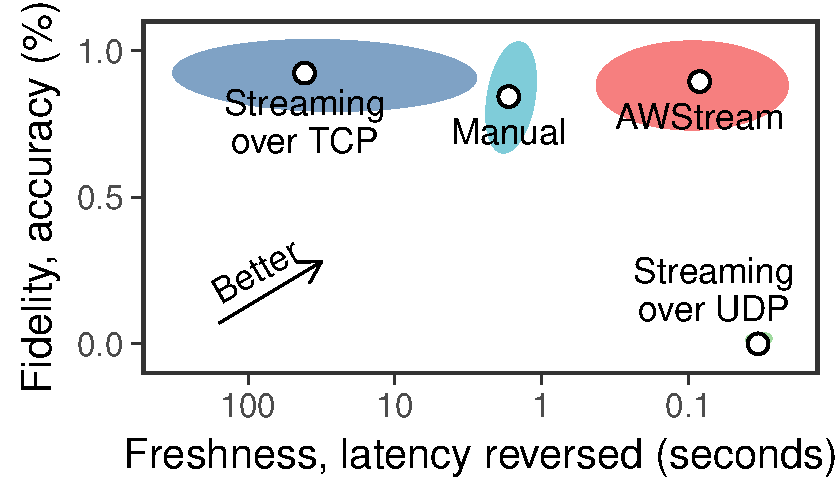
\includegraphics[width=0.9\columnwidth]{figures/figure1.pdf}
  \caption{The trade-off space between data freshness and fidelity when facing
    insufficient bandwidth (details in \autoref{sec:runtime-adaptation}).}
  \label{fig:intro}
  \vspace{-1em}
\end{figure}

Applications using existing protocols without adaptation result in extreme
design points. Streaming over TCP ensures a reliable delivery but backlogged
data increases latency. On the other hand, streaming over UDP minimizes latency
by sending packets as fast as possible, but uncontrolled loss devastates
application accuracy.

Manual policies, such as sampling, allow developers to trade data fidelity for
freshness~\cite{rabkin2014aggregation}. However, it's difficult to write
accurate policies without extensive expertise or without considerable
efforts. In practice, developers write manual policies based on heuristics
rather than quantitative measurements. These inaccurate policies lead to
sub-optimal performance for both freshness and fidelity.

Furthermore, application-specific optimizations do not generalize. A fine-tuned
adaptation algorithm for one application works poorly for a different
application, if performance metrics or data distributions change.  For example,
video streaming focuses on quality of experience
(QoE)~\cite{michalos2012dynamic, pantos2016http, yin2015control}. Because humans
favor smoothness over image quality, these systems maintain a high frame rate,
e.g.\,\(25~\text{FPS}\), and reduce the resolution under bandwidth limitation.
Low resolution images lead to poor accuracy for analytic jobs that rely on image
details.

In this paper, we design and implement \sysname{}, a stream processing system
for the wide area that achieves low latency and high accuracy simultaneously
with minimal developer effort. The key idea is to automatically build an
accurate and precise performance model instead of relying on manual policies or
application-specific optimizations. \sysname{}'s solution is three-fold:
easy-to-use APIs, automatic profiling, and a low-latency runtime.

\sysname{} augments existing stream processing operators with a new \maybe{}
operator. Its basic form takes a list of values as a knob and a function that
degrades the input stream. The knob specifies the degradation level that affects
data size and data fidelity. We extend the basic form with a library of
specialized operators for common data types, such as \texttt{maybe\_downsample}
for images. Our APIs are simple, composable and extensible. Developers do not
need to be an expert in the application domain as the knobs tolerate approximate
specifications. Multiple operators form a configuration that affects the
adaptation jointly. Arbitrary functions and external libraries can be embedded
with our operators.

\sysname{} then uses a data-driven approach to automatically build application
performance profiles with minimal developer effort. The profiles accurately
capture the relationship between application accuracy and bandwidth consumption
under different combinations of data degradation operations. We use an offline
process to bootstrap our system with developer-supplied training data, and
continuously refine the profile online to handle model drifts. We exploit
parallelism and sampling-based profiling to efficiently explore the
configuration space and learn a Pareto-optimal adaptation strategy.

At runtime, \sysname{} achieves low latency by matching data rate to available
bandwidth, and high accuracy by using Pareto-optimal configurations from the
profile. Upon network congestion, our rate adaptation algorithm increases the
degradation level to reduce data rate, such that no persistent queue builds
up. To recover, it progressively decreases the degradation level after probing
for more available bandwidth. The runtime also provides additional options to
control application behaviors, such as limiting the maximum allowed WAN
bandwidth. For multiple applications, the profiles can be used to allocate
bandwidth among competing tasks for utility fairness.

To evaluate \sysname{}, we have built three streaming applications: augmented
reality (AR), pedestrian detection (PD), and distributed Top-K (TK). We use
real-world data to profile these applications and evaluate their runtime
performance on a geo-distributed public cloud. Our contributions and evaluation
results are as follows.

\begin{itemize}[leftmargin=*, topsep=2pt, itemsep=2pt]

\item We propose \maybe{} operators to incorporate adaptation with existing
  stream processing models. Our programming abstraction is simple, composable
  and extensible.

\item We show that \sysname{}'s data-driven approach generates an accurate and
  precise profile for each application. Parallelism and sampling techniques
  can speed up the profiling substantially, up to 29$\times$ and 9$\times$\@.

\item Using runtime experiments on geo-distributed EC2 nodes, \sysname{}
  achieves low latency and high accuracy simultaneously for all
  applications---sub-second latency and nominal accuracy drop (2-3\%).

\end{itemize}

%%% Local Variables:
%%% mode: latex
%%% TeX-master: "awstream"
%%% End:

%% LocalWords: VideoStorm, analytics, CDN, IoT
